\documentclass[11pt, oneside]{article} 
\usepackage{geometry}
\geometry{letterpaper} 
\usepackage{graphicx}
	
\usepackage{amssymb}
\usepackage{amsmath}
\usepackage{parskip}
\usepackage{color}
\usepackage{hyperref}

\graphicspath{{/Users/telliott_admin/Tex/png/}}
% \begin{center} \includegraphics [scale=0.4] {gauss3.png} \end{center}

\title{Higher derivatives}
\date{}

\begin{document}
\maketitle
\Large
We have defined the derivative of a function $f(x)$ as a limit
\[  \lim_{h \to 0} \  \frac{f(x+h) - f(x)}{h} \]

It is the limit of the difference quotient as $h \rightarrow 0$.

We introduced the power rule to obtain the derivative of integer powers of $x$.  In addition, we said that the derivative of a sum of two or more functions is the sum of the derivatives.

The derivative is just a function itself.  Consider a quadratic like
\[ y = ax^2 + bx + c \]
The derivative is
\[ y' = 2ax + b \]

Since the derivative is just a function, why not take the derivative of the derivative, which is called
\[ \frac{d^2y}{dx^2} \]
or more compactly, $y$ double prime:
\[ y'' = 2a \]

What is the meaning of the second derivative?  It gives the slope of the slope, or how the slope is changing with a change in $x$.  For a parabola that opens up, like this one
\begin{center} 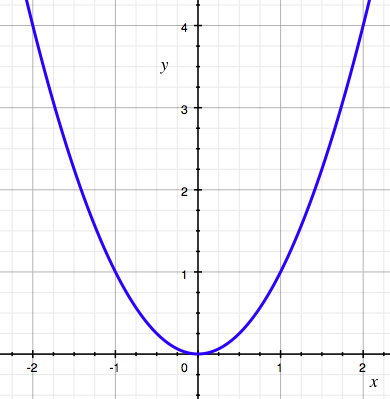
\includegraphics [scale=0.4] {para5.png} \end{center}

the second derivative is positive.  This means that the slope continues to increase as $x$ increases.

There is nothing to stop us from taking more derivatives.  For a quadratic $y''' = 0$, which is not very interesting, but consider the cubic:
\[ y = x^3 \]
\[ y' = 3x^2 \]
\[ y'' = 6x \]
\[ y''' = 6 \]

\subsection*{extrema}

A very important use of the derivative is to find a maximum or minimum of a function.  At such a point the slope is zero because the curve is headed sideways, just for a moment.  For the quadratic, the slope is zero at the vertex:
\[ y' = 0 = 2ax + b \]
\[ x = -\frac{b}{2a} \]

You should recognize this equation from geometry.  Without getting into details, it is obtained there by completing the square.  Or alternatively, write the equation of a parabola whose vertex is $(h,k)$
\[ (y - k) = a(x - h)^2 \]
multiply out
\[ y = ax^2 - 2ahx + h^2 + k \]
By comparison with the standard form
\[ y = ax^2 + bx + c \]
it's clear that
\[ - 2ahx = bx \]
so the $x$-coordinate of the vertex is
\[ h = -\frac{b}{2a} \]

The vertex is the maximum or minimum of a quadratic, depending on the sign of $a$.  We can tell the difference by looking at the second derivative again:
\[ y'' = 2a \]
If $a > 0$ (a parabola that opens up), then the second derivative is positive and we have found a minimum value.  If $y'' < 0$, we have a maximum.

Consider the cubic 
\[ y = (x+1)(x+1)(x-1) \]
\[ = (x^2 + 2x + 1)(x - 1) \]
\[ = x^3 + x^2 - x - 1 \]

From the first form, we can easily see that the roots are $x = \pm \ 1$.  These are the values where the function crosses the $y$-axis, that is, where its value is zero.

The graph looks like this:
\begin{center} 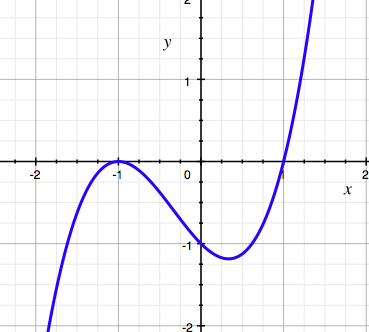
\includegraphics [scale=0.4] {cubic_simple.png} \end{center}
The first derivative is
\[ y' = 3x^2 + 2x - 1 \]
\[ = (3x - 1)(x + 1) \]
This expression is zero when $x = -1$ or $x = 1/3$.  That does match the places where the curve is horizontal, as we can see.

The second derivative is
\[ y'' = 6x + 2 \]

For the first value $x = -1$, the second derivative is negative, and this corresponds to a local maximum for the function.  For $x = 1/3$, the second derivative is positive, and this is a minimum.  We say "local" because there may be more extreme values, as is the case here.

A maximum corresponds to a negative value for the slope of the slope because the slope is first positive, then zero, then negative.  Its change with increasing $x$ is negative.

Again, the second derivative of our cubic is
\[ y'' = 6x + 2 \]
Setting this equal to zero, we obtain
\[ x = - \frac{1}{3} \]
This point on the curve is an \emph{inflection point}.  It is a point (actually the only point for this curve) where the rate of change of the slope, which is negative to the left $x = -1/3$, changes to positive, and there is an instant where it is zero.

\begin{center} 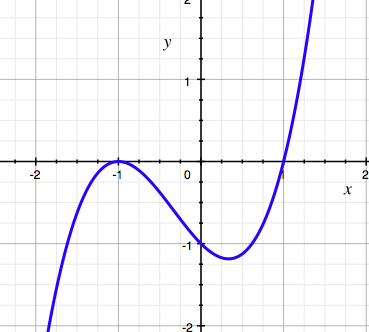
\includegraphics [scale=0.4] {cubic_simple.png} \end{center}

We will see this in connection with the Gaussian or normal curve.  It's an interesting fact that the first standard deviation corresponds to the inflection point of the curve.  At that point the second derivative of the function is equal to zero.

\subsection*{Rectangular area}
Here is a classic problem.

We wish to construct a rectangle with the maximum area \emph{for a fixed perimeter} (without the second statement the area would be infinite).  Let's call the sides $x$ and $y$, and the semi-perimeter $S$ (constant) and so our constraint is that 
\[ S = x + y \]
The area is then
\[ A = xy \]
substitute
\[ A = x (S - x) \]
\[ = Sx - x^2 \]

Take the first derivative and set it equal to zero:
\[ A' = S - 2x = 0 \]
\[ x = \frac{S}{2} = y \]
A square has the maximum area for a given perimeter constructed with right angles, as expected.  We'll see many challenging problems of this type later on.

\end{document}